% Options for packages loaded elsewhere
\PassOptionsToPackage{unicode}{hyperref}
\PassOptionsToPackage{hyphens}{url}
\documentclass[
  ignorenonframetext,
]{beamer}
\newif\ifbibliography
\usepackage{pgfpages}
\setbeamertemplate{caption}[numbered]
\setbeamertemplate{caption label separator}{: }
\setbeamercolor{caption name}{fg=normal text.fg}
\beamertemplatenavigationsymbolsempty
% remove section numbering
\setbeamertemplate{part page}{
  \centering
  \begin{beamercolorbox}[sep=16pt,center]{part title}
    \usebeamerfont{part title}\insertpart\par
  \end{beamercolorbox}
}
\setbeamertemplate{section page}{
  \centering
  \begin{beamercolorbox}[sep=12pt,center]{section title}
    \usebeamerfont{section title}\insertsection\par
  \end{beamercolorbox}
}
\setbeamertemplate{subsection page}{
  \centering
  \begin{beamercolorbox}[sep=8pt,center]{subsection title}
    \usebeamerfont{subsection title}\insertsubsection\par
  \end{beamercolorbox}
}
% Prevent slide breaks in the middle of a paragraph
\widowpenalties 1 10000
\raggedbottom
\AtBeginPart{
  \frame{\partpage}
}
\AtBeginSection{
  \ifbibliography
  \else
    \frame{\sectionpage}
  \fi
}
\AtBeginSubsection{
  \frame{\subsectionpage}
}
\usepackage{iftex}
\ifPDFTeX
  \usepackage[T1]{fontenc}
  \usepackage[utf8]{inputenc}
  \usepackage{textcomp} % provide euro and other symbols
\else % if luatex or xetex
  \usepackage{unicode-math} % this also loads fontspec
  \defaultfontfeatures{Scale=MatchLowercase}
  \defaultfontfeatures[\rmfamily]{Ligatures=TeX,Scale=1}
\fi
\usepackage{lmodern}
\ifPDFTeX\else
  % xetex/luatex font selection
\fi
% Use upquote if available, for straight quotes in verbatim environments
\IfFileExists{upquote.sty}{\usepackage{upquote}}{}
\IfFileExists{microtype.sty}{% use microtype if available
  \usepackage[]{microtype}
  \UseMicrotypeSet[protrusion]{basicmath} % disable protrusion for tt fonts
}{}
\makeatletter
\@ifundefined{KOMAClassName}{% if non-KOMA class
  \IfFileExists{parskip.sty}{%
    \usepackage{parskip}
  }{% else
    \setlength{\parindent}{0pt}
    \setlength{\parskip}{6pt plus 2pt minus 1pt}}
}{% if KOMA class
  \KOMAoptions{parskip=half}}
\makeatother
\usepackage{longtable,booktabs,array}
\newcounter{none} % for unnumbered tables
\usepackage{calc} % for calculating minipage widths
\usepackage{caption}
% Make caption package work with longtable
\makeatletter
\def\fnum@table{\tablename~\thetable}
\makeatother
\usepackage{graphicx}
\makeatletter
\newsavebox\pandoc@box
\newcommand*\pandocbounded[1]{% scales image to fit in text height/width
  \sbox\pandoc@box{#1}%
  \Gscale@div\@tempa{\textheight}{\dimexpr\ht\pandoc@box+\dp\pandoc@box\relax}%
  \Gscale@div\@tempb{\linewidth}{\wd\pandoc@box}%
  \ifdim\@tempb\p@<\@tempa\p@\let\@tempa\@tempb\fi% select the smaller of both
  \ifdim\@tempa\p@<\p@\scalebox{\@tempa}{\usebox\pandoc@box}%
  \else\usebox{\pandoc@box}%
  \fi%
}
% Set default figure placement to htbp
\def\fps@figure{htbp}
\makeatother
\setlength{\emergencystretch}{3em} % prevent overfull lines
\providecommand{\tightlist}{%
  \setlength{\itemsep}{0pt}\setlength{\parskip}{0pt}}
% Slide layout defaults for warning-clean scientific decks.
\usepackage{etoolbox}
\IfFileExists{xurl.sty}{\usepackage{xurl}}{}
\IfFileExists{seqsplit.sty}{\usepackage{seqsplit}}{\newcommand{\seqsplit}[1]{#1}}
\protected\def\breakseq#1{\seqsplit{#1}}
\protected\def\breaktt#1{\begingroup\ttfamily\seqsplit{#1}\endgroup}
\setlength{\emergencystretch}{6em}
\tolerance=5000
\hbadness=10000
\hfuzz=1pt
\setlength{\tabcolsep}{2pt}
\AtBeginEnvironment{longtable}{\tiny\renewcommand{\arraystretch}{0.86}\setlength{\tabcolsep}{1pt}}
\AtBeginEnvironment{tabular}{\tiny\renewcommand{\arraystretch}{0.86}\setlength{\tabcolsep}{1pt}}

% Natbib and cross-reference fallbacks — slides don't load natbib
% or cleveref, but combined-PDF manuscript prose may emit these
% commands. The fallback renders citations as a bracketed key list
% and cross-references as detokenized labels so slides don't fail on
% undefined control sequences or raw underscores. \providecommand is
% a no-op if packages load later.
\providecommand{\citep}[1]{[#1]}
\providecommand{\citet}[1]{#1}
\providecommand{\citealp}[1]{#1}
\providecommand{\citeauthor}[1]{#1}
\providecommand{\citeyear}[1]{#1}
\providecommand{\cref}[1]{\texttt{\detokenize{#1}}}
\providecommand{\Cref}[1]{\texttt{\detokenize{#1}}}
\usepackage{bookmark}
\IfFileExists{xurl.sty}{\usepackage{xurl}}{} % add URL line breaks if available
\urlstyle{same}
% fallback for those not using the hyperref driver hyperxmp:
\makeatletter
\@ifundefined{xmpquote}{\newcommand{\xmpquote}[1]{#1}}{}
\makeatother
\hypersetup{
  hidelinks,
  pdfcreator={LaTeX via pandoc}}

\author{\texorpdfstring{}{}}
\date{}

\begin{document}

\section{Methods: instrument, assumptions, and companion
track}\label{methods-instrument-assumptions-and-companion-track}

\begin{frame}[fragile,allowframebreaks]{Synthetic deterministic track:
seeded panels, blind estimates, oracle scoring}
\protect\phantomsection\label{synthetic-deterministic-track-seeded-panels-blind-estimates-oracle-scoring}
The first methodological track is a seeded synthetic instrument. It
generates known populations and corpora, hides the answer key from the
\texttt{ntqr} estimator, and then scores the returned logically
consistent evaluations against the supervised oracle that is available
only because the data are synthetic.

\begin{block}{Pipeline: panel formation precedes no-answer-key
estimation}
\protect\phantomsection\label{pipeline-panel-formation-precedes-no-answer-key-estimation}
The instrument runs strictly upstream-to-downstream and is deterministic
end to end (every stochastic step is seeded with
\breaktt{numpy.random.default\_rng}; figures use
\texttt{MPLBACKEND=Agg}). One \textbf{trial} is:

\begin{enumerate}
\tightlist
\item
  \textbf{Generate} a synthetic expert population of known properties.
\item
  \textbf{Form} a panel from that population with one of four
  strategies.
\item
  \textbf{Judge} a corpus of items whose ground-truth labels are
  \emph{known to us but hidden from the estimator}.
\item
  \textbf{Evaluate} the panel with the \texttt{ntqr} package
  \emph{without the answer key}.
\item
  \textbf{Score} the unsupervised estimate against the supervised
  \textbf{oracle} computed from the known labels.
\end{enumerate}

\breakseq{[@fig:pipeline]} shows this upstream-to-downstream flow at a glance.

\begin{figure}
\centering
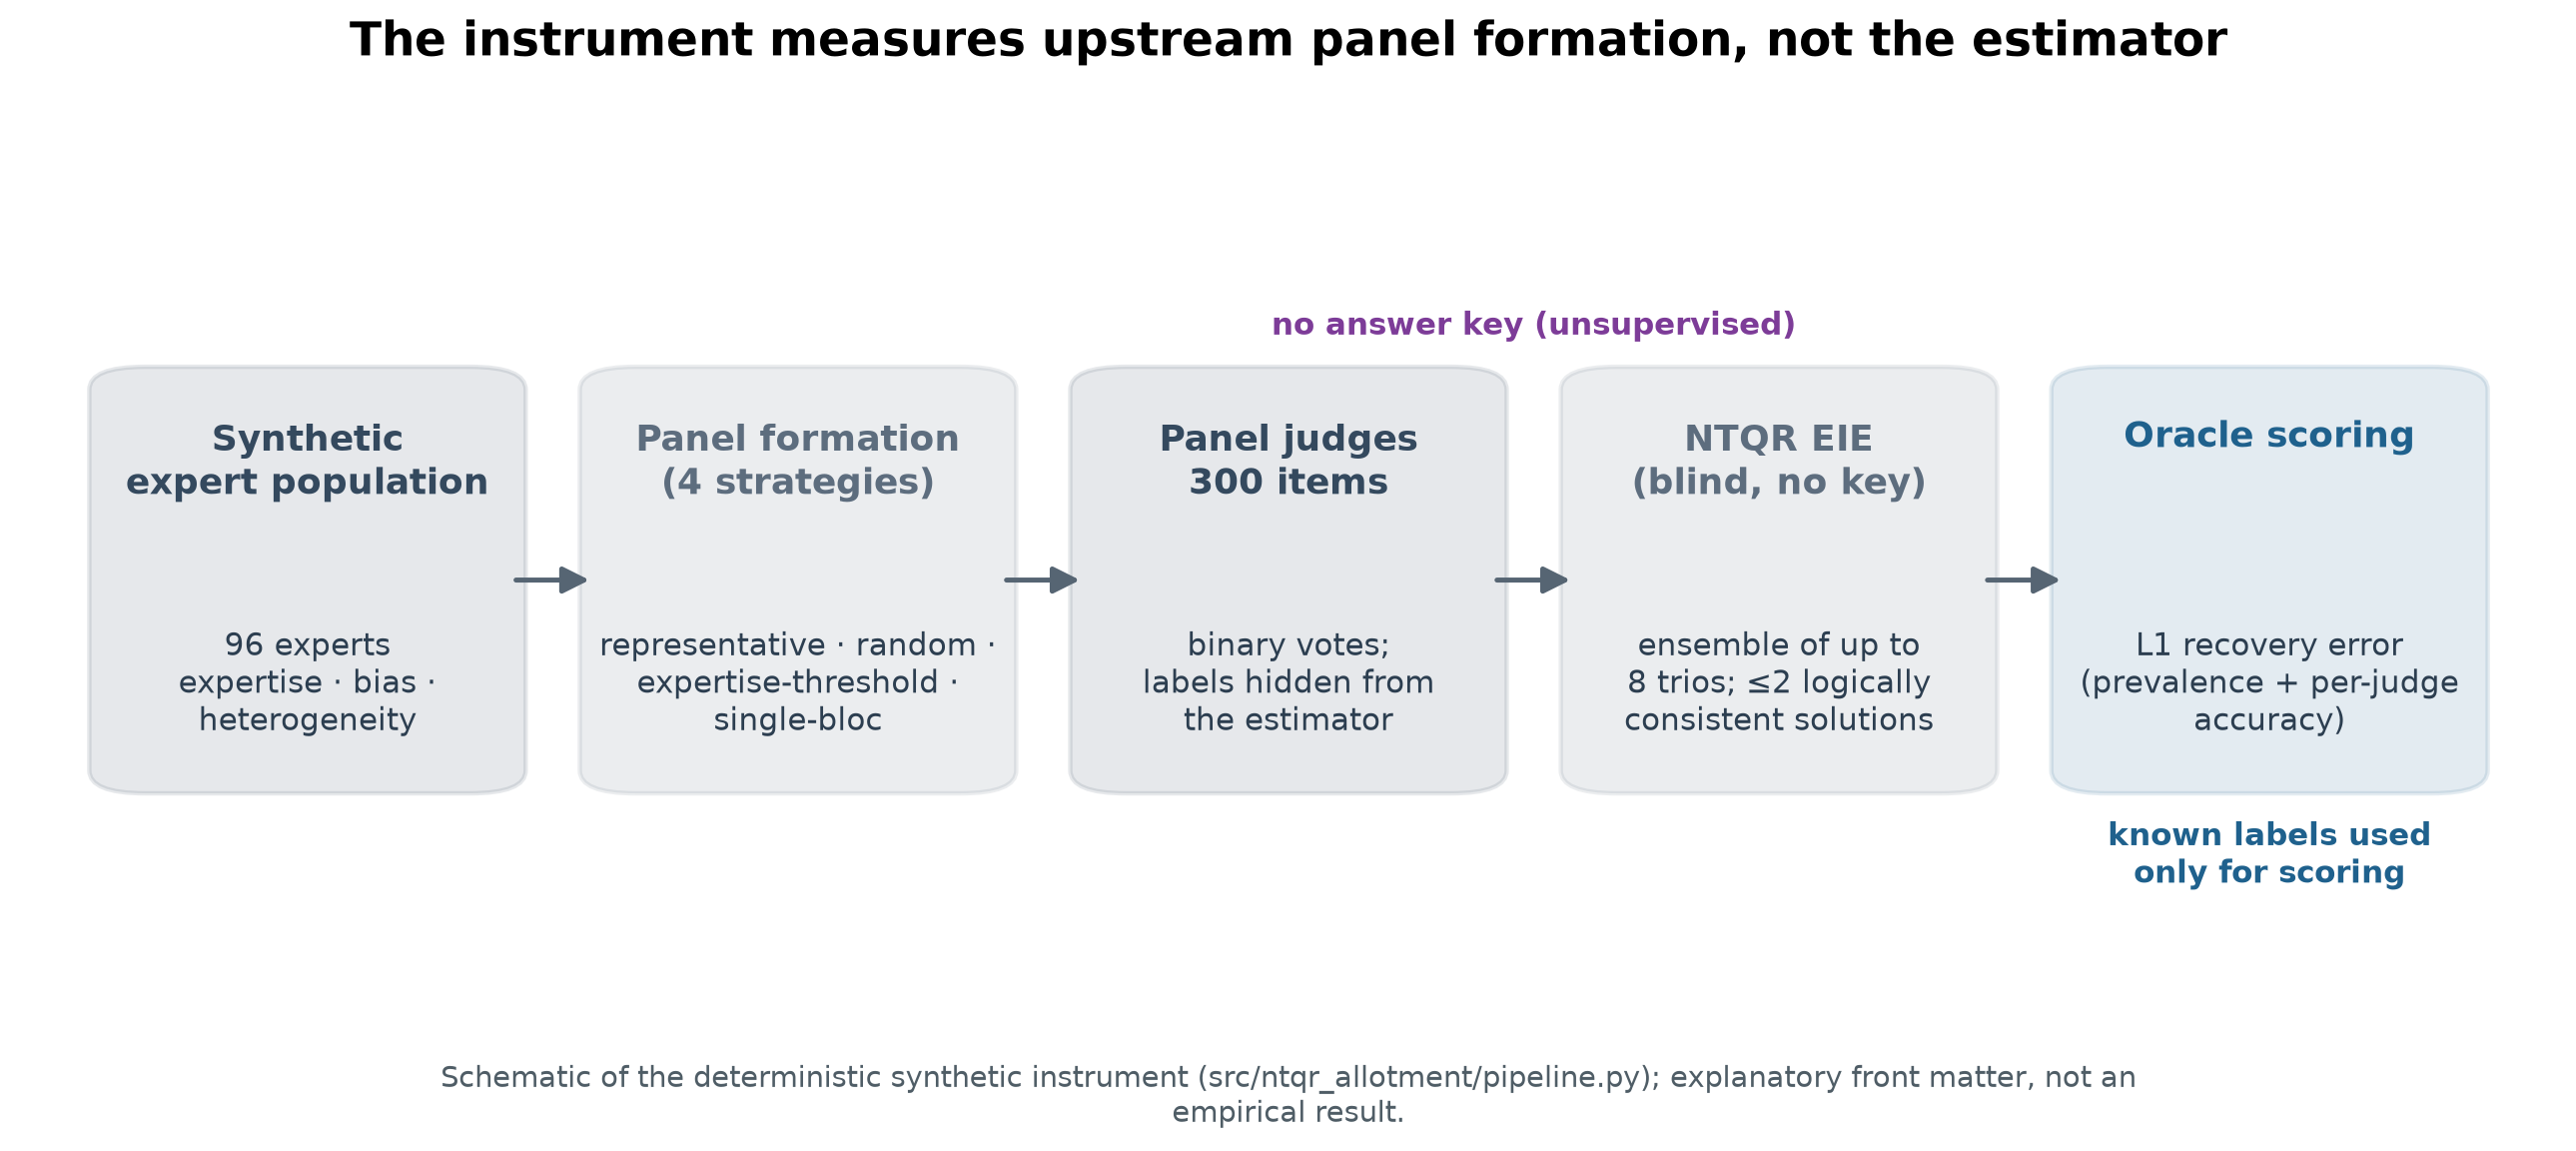
\includegraphics[width=0.95\linewidth,height=0.46\textheight,keepaspectratio,alt={Left-to-right pipeline of the deterministic synthetic instrument (steps 1--5 in text; count tokens annotated from 96, 300, 8 so the figure cannot drift from the reported configuration): a known population is sampled → a panel is formed by one of four strategies → the panel judges a key-hidden corpus → the EIE evaluator runs blind over trios → only scoring reads the labels. The bracket marks the unsupervised region; the manipulated variable is the upstream formation rule. Explanatory schematic only; quantitative results are in the Results section.}]{../figures/method_pipeline_schematic.png}
\caption{Left-to-right pipeline of the deterministic synthetic
instrument (steps 1--5 in text; count tokens annotated from
\protect\texttt{96}, \protect\texttt{300}, \protect\texttt{8} so the
figure cannot drift from the reported configuration): a known population
is sampled → a panel is formed by one of four strategies → the panel
judges a key-hidden corpus → the EIE evaluator runs blind over trios →
only scoring reads the labels. The bracket marks the unsupervised
region; the manipulated variable is the upstream formation rule.
Explanatory schematic only; quantitative results are in the Results
section.}\label{fig:pipeline}
\end{figure}

The key methodological move is step 5: because the ground truth is
synthetic and therefore known, the unlabeled \texttt{ntqr} evaluation
and the supervised oracle can be compared on equal footing. Recovery
error is the L1-style distance between the two evaluations --- the
absolute prevalence error plus the mean absolute per-judge accuracy
error. Throughout, ``ground-truth-free'' is project shorthand for this
no-answer-key estimator path, not an expansion or alternative name for
\texttt{ntqr}.

\textbf{Synthetic expert population.} Each expert is a noisy binary
judge with label-conditional accuracies
\texttt{accuracy\_a\ =\ P(vote\ a\ \textbar{}\ true\ a)} and
\texttt{accuracy\_b\ =\ P(vote\ b\ \textbar{}\ true\ b)}, derived from a
continuous \texttt{expertise} (mean precision) and a signed
\texttt{bias} that skews errors toward one label. The population sampler
draws expertise from a normal centered at \texttt{mean\_expertise} with
standard deviation \breaktt{expertise\_heterogeneity}, and draws bias
with a sign \textbf{correlated with each expert's ideology} (left →
negative, right → positive). Because this only shifts each judge's
\emph{marginal} accuracy by ideology --- every judge still errs from an
independent stream --- it does not by itself make single-bloc panels
more error-correlated than a representative draw; supplying that missing
cross-judge error-correlation channel is the job of the
composition-coupled confound introduced below. Each population in the
sweep has 96 experts; each corpus has 300 items sampled at the
configured prevalence.
\end{block}

\begin{block}{Panel-formation strategies: four upstream rules}
\protect\phantomsection\label{panel-formation-strategies-four-upstream-rules}
All four strategies are deterministic given their seed.

\begin{itemize}
\tightlist
\item
  \textbf{representative\_sortition} --- an auditable maximin lottery
  implemented on the open-source \texttt{allotment} engine
  (\href{https://github.com/Citizen-Infra/allotment}{Citizen-Infra
  (2024)}, the AGPL-3.0 sortition library this project imports and uses
  directly), which realizes the fair stratified-selection algorithm of
  \href{https://doi.org/10.1038/s41586-021-03788-6}{Flanigan et
  al.~(2021)}. Ideology quotas are set by largest-remainder (Hamilton)
  apportionment so the panel mirrors the population's ideology
  composition as closely as integer seats allow; the draw carries the
  engine's SHA-256 audit hash for reproducibility.
\item
  \textbf{random\_selection} --- a uniform draw without replacement.
  This is the simplest honest baseline and is treated as a first-class
  comparator throughout.
\item
  \textbf{ideological\_selection} --- fill the panel from a single
  ideology bloc first, spilling over only if the bloc is too small. This
  deliberately concentrates correlated biases and is the
  \emph{non-representative} comparator.
\item
  \textbf{expertise\_threshold} --- select the top-k experts by
  expertise. This is the competence-first comparator and ignores
  representativeness entirely.
\end{itemize}
\end{block}

\begin{block}{NTQR evaluation: trio EIE, oracle scoring, and majority
voting}
\protect\phantomsection\label{ntqr-evaluation-trio-eie-oracle-scoring-and-majority-voting}
The \texttt{ntqr} package's exact error-independent evaluator is
\textbf{trio-only}: it solves the error-independent algebraic system for
\emph{exactly three} binary judges, returning logically consistent
(prevalence, per-judge accuracy) evaluations. The system admits up to
two real solutions; complex or non-finite roots are dropped honestly
rather than coerced. To resolve the two-fold ambiguity in the synthetic
track we select the consistent solution \textbf{closest to the oracle}
--- this is the most charitable reading of the unlabeled estimate, so
any residual error is a real failure to match the supervised oracle, not
a sign ambiguity.

We compute two \texttt{ntqr} evaluations per trio: the error-independent
evaluation (EIE, our headline) and the majority-voting evaluation (a
comparator that partitions solutions into crowd-right and crowd-wrong).
The \textbf{supervised oracle} is read directly from the
label-conditioned vote counts; it is always real and finite, and a
degenerate oracle is treated as a contract violation that fails loudly.

\textbf{Ensemble-of-trios for panels larger than three.} Because the
exact solver is trio-only, a panel of size greater than three is
evaluated by \textbf{ensemble-of-trios}. We scan trios (combinations of
panel members) in deterministic order, collecting up to 8 \emph{usable}
trios --- a trio is skipped if its vote pattern admits no real
error-independent solution --- and average their oracle-referenced
errors. A single bad expert therefore does not starve the ensemble. If
\emph{every} trio in a panel is degenerate, the trial records an honest
NaN (zero usable trios) so a sweep surfaces ``no recovery possible
here'' rather than crashing or inventing a number. A panel of exactly
three reduces to a single trio, so the ensemble result coincides with
the single-trio result there.

Historically, Borda- and Condorcet-style work asks how votes should be
aggregated once a voting body exists; here, the formation rule is part
of the experimental treatment. The Methods therefore keep two objects
separate throughout: the upstream panel draw and the downstream
no-answer-key estimator.
\end{block}

\begin{block}{Companion diagnostics: alarm cost, ternary feasibility,
and maximin fairness}
\protect\phantomsection\label{companion-diagnostics-alarm-cost-ternary-feasibility-and-maximin-fairness}
Three companion tracks measure structural properties of the instrument
rather than oracle-referenced recovery error.

\textbf{Alarm scaling is a small-\(Q\) constraint.} The \texttt{ntqr}
package also ships an \textbf{alarm}: it tests whether all judges can be
simultaneously consistent with some answer key at a stated safety
specification, a constraint system that gains more panel-size-indexed
checks as judges are added. Unlike the trio evaluator, this project's
alarm path enumerates the answer-key simplex, and our local benchmark
shows roughly \textbf{cubic scaling in the corpus size \(Q\)}. A shipped
benchmark (\breaktt{scripts/bench\_alarm.py}) reproduces this scaling on
demand; indicative single-machine timings rise from about 0.7 s at
\(Q=20\) to 8.9 s at \(Q=50\) to 97.9 s at \(Q=100\) (the exact
constants vary with machine load --- the cubic \emph{scaling}, not the
constants, is the robust local finding). This \(O(Q^3)\) cost is a
scaling limit on the statistical-power / alarm track as implemented
here, so we report it as a finding and cap any alarm use at \(Q\leq30\)
(opt-in only); larger corpora must raise the cap deliberately.

\textbf{The ternary \(R=3\) axiom-consistency track (consistency only).}
A companion track (\breaktt{src/ntqr\_allotment/ternary.py}) extends the
axiomatic surface from binary (\(R=2\)) to ternary (\(R=3\)) responses,
but \textbf{only at the level of axiom-consistency and feasibility ---
never \(R=3\) recovery}. It checks whether an observed three-way vote
profile is \emph{consistent} with the NTQR algebraic axioms (the
response counts sum correctly and lie in the feasible simplex), not
whether the unsupervised (prevalence, accuracy) state can be
\emph{solved}. Exact \(R=3\) recovery is unsolved upstream and is
explicitly \textbf{out of scope / anti-vision} for this work: we make no
claim to recover ternary evaluations. The track exists so the
consistency/feasibility axioms can be exercised and tested at \(R=3\)
without overstating what NTQR can do there.

\textbf{N-judge alarm power is consistency-only.} A second companion
track (\breaktt{src/ntqr\_allotment/ensemble.py}) generalizes the
single-trio consistency check to an \textbf{N-judge} observed-vote-count
alarm and measures how the consistency signal scales with panel size
(\breaktt{alarm\_power\_curve}). In the current small-\(Q\) diagnostic,
the tight safety setting is already saturated across the plotted panel
sizes, so the figure demonstrates that the N-judge alarm is executable
and panel-size-indexed rather than establishing a monotone growth law.
The underlying answer-key enumeration is the same \(O(Q^3)\) cost
described above, so the N-judge track is exercised only at \textbf{small
\(Q\)}. It is a panel-size-indexed \emph{consistency} signal, not a
recovery method.

\textbf{Maximin fairness is a selection metric.} The
representative-sortition strategy is an auditable maximin lottery, and a
fairness track (\breaktt{src/ntqr\_allotment/fairness.py}) characterizes
the allotment's \textbf{selection-probability distribution} over the
population --- the probability each expert is seated across the lottery.
The maximin objective is the \textbf{minimum selection probability}: a
fairer lottery raises the floor on who can be seated. This track
measures the representation properties of the draw itself and is
independent of the downstream NTQR recovery numbers.
\end{block}

\begin{block}{Notation: cells, trios, and inferential units}
\protect\phantomsection\label{notation-cells-trios-and-inferential-units}
The manuscript keeps each statistic tied to the unit that generated it;
this is the guardrail that prevents synthetic, power, and live empirical
claims from borrowing strength from one another. Table @tbl:notation is
the compact ledger for symbols, estimators, inferential units, and
artifact ownership.

\begin{longtable}[]{@{}
  >{\raggedright\arraybackslash}p{(\linewidth - 8\tabcolsep) * \real{0.2000}}
  >{\raggedright\arraybackslash}p{(\linewidth - 8\tabcolsep) * \real{0.2000}}
  >{\raggedright\arraybackslash}p{(\linewidth - 8\tabcolsep) * \real{0.2000}}
  >{\raggedright\arraybackslash}p{(\linewidth - 8\tabcolsep) * \real{0.2000}}
  >{\raggedright\arraybackslash}p{(\linewidth - 8\tabcolsep) * \real{0.2000}}@{}}
\caption{Notation and inferential units for the manuscript's reported
statistics.}\label{tbl:notation}\tabularnewline
\toprule\noalign{}
\begin{minipage}[b]{\linewidth}\raggedright
Symbol
\end{minipage} & \begin{minipage}[b]{\linewidth}\raggedright
Surface / estimator
\end{minipage} & \begin{minipage}[b]{\linewidth}\raggedright
Unit
\end{minipage} & \begin{minipage}[b]{\linewidth}\raggedright
Aggregation and uncertainty
\end{minipage} & \begin{minipage}[b]{\linewidth}\raggedright
Source artifact
\end{minipage} \\
\midrule\noalign{}
\endfirsthead
\toprule\noalign{}
\begin{minipage}[b]{\linewidth}\raggedright
Symbol
\end{minipage} & \begin{minipage}[b]{\linewidth}\raggedright
Surface / estimator
\end{minipage} & \begin{minipage}[b]{\linewidth}\raggedright
Unit
\end{minipage} & \begin{minipage}[b]{\linewidth}\raggedright
Aggregation and uncertainty
\end{minipage} & \begin{minipage}[b]{\linewidth}\raggedright
Source artifact
\end{minipage} \\
\midrule\noalign{}
\endhead
\(E, Q, \pi\) & Experts, items, and label prevalence hidden from NTQR &
one seeded population/corpus & profile metadata, config hash, seed list
& \breaktt{output/data/sweep\_results.json} \\
\(V_{ij}\) & Binary vote matrix by panel member \(i\) and item \(j\) &
one panel trial & supervised oracle retained only for scoring &
\breaktt{src/ntqr\_allotment/pipeline.py} \\
\(\widehat{\theta}_{\mathrm{EIE}}\) & NTQR error-independent evaluation
& one usable trio & oracle-referenced recovery error &
\breaktt{src/ntqr\_allotment/ntqr\_eval.py} \\
\(\bar{e}_{\mathrm{trio}}\) & Ensemble aggregation over usable trios &
up to 8 trios per panel & NaN/sentinel if every trio is degenerate &
\breaktt{output/data/sweep\_aggregated.csv} \\
\(\bar{e}_{s}\) & Strategy ranking by weighted mean EIE error & strategy
over active profile cells & pooled 95\% CI, seed count, profile/hash &
\breaktt{output/data/sweep\_aggregated.csv} \\
\(\Delta_{\mathrm{ideo-rep}}\) & Ideological-minus-representative
contrast & active-profile regime cells & observed-vs-predicted
alignment, descriptive intervals &
\breaktt{output/data/analytical\_predictions.json} \\
\(\rho_{\mathrm{NTQR}}\) & Realized pairwise error correlation &
non-degenerate (\(\rho\), strategy) cell & OLS slope with bootstrap CI
over unique cells & \breaktt{output/data/independence\_sweep.csv} \\
\(d, n, \mathrm{MDE}\) & Two-sample power design quantities &
per-strategy EIE observations at fixed panel size & Cohen's \(d\),
permutation \(p\), Holm correction, MDE, per-group observation budget &
\breaktt{output/data/power\_analysis.csv} \\
\(\Delta_{\mathrm{age}}\) & Live postdoctoral-review age-disparity
stress test & strategy x panel-size under one Gemma model &
older-minus-younger recommendation-rate difference, descriptive
intervals & \breaktt{output/data/postdoc\_panel\_results.json} \\
\(A_{\mathrm{align}}\) & Analytical-vs-Gemma postdoc alignment &
strategy x panel-size cells & directional sign agreement and
unresolved-cell count &
\breaktt{output/data/postdoc\_panel\_alignment.json} \\
\bottomrule\noalign{}
\end{longtable}
\end{block}

\begin{block}{Assumption ledger: how each claim can fail}
\protect\phantomsection\label{assumption-ledger-how-each-claim-can-fail}
The analysis is organized as falsifiable claims rather than a single
success story. Table @tbl:falsification states what would count against
each claim and which artifact carries the check. The rows map onto the
Introduction's hypotheses: the representative-vs-ideological,
panel-size, tolerance-sweep, and real-Ollama rows are the
negative-control checks for H2, H3, H4, and H5 respectively; the
NTQR-EIE-recovery row guards the estimator the whole study depends on
(and so underpins H1, the strategy ranking tested directly in Results);
and the null-and-significance row fixes the design-limited-vs-resolved
interpretation discipline applied throughout.

\begin{longtable}[]{@{}
  >{\raggedright\arraybackslash}p{(\linewidth - 6\tabcolsep) * \real{0.2500}}
  >{\raggedright\arraybackslash}p{(\linewidth - 6\tabcolsep) * \real{0.2500}}
  >{\raggedright\arraybackslash}p{(\linewidth - 6\tabcolsep) * \real{0.2500}}
  >{\raggedright\arraybackslash}p{(\linewidth - 6\tabcolsep) * \real{0.2500}}@{}}
\caption{Assumption and falsification ledger for the manuscript's main
claim families.}\label{tbl:falsification}\tabularnewline
\toprule\noalign{}
\begin{minipage}[b]{\linewidth}\raggedright
Claim family
\end{minipage} & \begin{minipage}[b]{\linewidth}\raggedright
Load-bearing assumption
\end{minipage} & \begin{minipage}[b]{\linewidth}\raggedright
Negative-control or falsification check
\end{minipage} & \begin{minipage}[b]{\linewidth}\raggedright
Current interpretation
\end{minipage} \\
\midrule\noalign{}
\endfirsthead
\toprule\noalign{}
\begin{minipage}[b]{\linewidth}\raggedright
Claim family
\end{minipage} & \begin{minipage}[b]{\linewidth}\raggedright
Load-bearing assumption
\end{minipage} & \begin{minipage}[b]{\linewidth}\raggedright
Negative-control or falsification check
\end{minipage} & \begin{minipage}[b]{\linewidth}\raggedright
Current interpretation
\end{minipage} \\
\midrule\noalign{}
\endhead
NTQR EIE recovery & The three-judge error-independent algebra is the
right estimator for a usable trio. & Complex/non-finite roots and
every-degenerate panels are retained as failures, not coerced into
numbers. & Residual recovery error is scored only after a real logically
consistent solution exists. \\
Representative-vs-ideological contrast & Bias concentration should
affect oracle-referenced EIE error through error dependence. & Cellwise
ideological-minus-representative heatmap plus analytical directional
checks can disagree with the predicted sign. & Design-limited on the
baseline grid (independent errors); resolved once the
composition-coupled confound supplies the error channel
(\breakseq{[@fig:blocphase]}), not a universal sortition win. \\
Panel size & Enlarging the panel averages more trios; whether that helps
or hurts, and by what mechanism, is measured rather than assumed. &
Paired per-strategy size contrast can show error rising with panel size;
the per-trio diagnostic locates the cause. & The active profile
falsifies a uniform ``larger is better'' rule and refutes the
error-correlation explanation for it. \\
Tolerance sweep & Injected \(\rho\) should be visible in NTQR-measured
realized error correlation. & The measured \(\rho_{\mathrm{NTQR}}\) must
rise with injected \(\rho\) before any recovery-slope story is
considered. & The diagnostic works; the recovery slope is unresolved
under global injection but resolves positive under the
marginal-preserving composition-coupled instrument
(\breakseq{[@fig:blocphase]}). \\
Real-Ollama postdoc companion & The same sampling mechanism should shape
age-bias expression and ranking under one prompted local LLM. &
Gemma-only reviewer-panel rows can disagree with the analytical sign or
remain unresolved by cell. & Reported as n-limited empirical companion
evidence, not human-review validation. \\
Null and significance language & A non-significant contrast is not
evidence of no effect unless the design could detect the relevant effect
size. & Permutation p-values, Holm correction, MDE, and sample-size
budgets are all reported together. & Nulls are split into resolved,
underpowered, and well-powered design statements. \\
\bottomrule\noalign{}
\end{longtable}
\end{block}

\begin{block}{Sweep profiles: profiles, seeds, and aggregation units}
\protect\phantomsection\label{sweep-profiles-profiles-seeds-and-aggregation-units}
The synthetic track is a deterministic grid sweep over the four
strategies, panel sizes, expert stringency, bias spread, and the
population/corpus parameters in \breaktt{manuscript/config.yaml}. That
file now defines named profiles: the reported sweep uses
\breaktt{manuscript\_contrast} (config hash \texttt{fda4da941cf0}), while
\texttt{smoke}, \texttt{manuscript\_main}, \texttt{tolerance},
\texttt{power}, \texttt{panel\_ladder}, and \texttt{research\_broad}
keep CI, legacy manuscript, assumption-tolerance, design-budget, finer
panel-size, and broader sensitivity settings explicit.
\breaktt{live\_postdoc\_panel} separately stores the required-live Gemma
model settings, reviewer/application counts, decode controls, and
vote-cache path. Each reported grid cell is repeated over 96 seeds; per
cell we report the mean EIE error, its sample standard deviation, and a
95\% confidence interval. Degenerate cells (no usable trio) are excluded
from aggregation via the same sentinel the emitter respects. A single
seed is treated as an illustration, never a finding --- all reported
effects are seed-aggregated with confidence intervals. The aggregated
table (\breaktt{output/data/sweep\_aggregated.csv}) and per-seed JSON
(\breaktt{output/data/sweep\_results.json}) carry the profile name,
config hash, seed list, and degenerate-row count; manuscript numbers are
emitted from those artifacts by
\breaktt{src/ntqr\_allotment/manuscript\_variables.py}, so no result is
hand-transcribed.
\end{block}

\begin{block}{Controlled-correlation sweep: injected dependence as a
diagnostic}
\protect\phantomsection\label{controlled-correlation-sweep-injected-dependence-as-a-diagnostic}
The error-independence assumption is probed directly.
\texttt{dependence.py}'s
\breaktt{sample\_votes\_correlated(experts,\ items,\ *,\ rho,\ seed)}
injects a controllable shared-error latent of strength \(\rho\), and
\breaktt{measure\_error\_correlations} reports the \emph{realized}
pairwise and three-way correlation NTQR itself computes from the votes
--- so the knob (\(\rho\)) and the measured quantity are independent.
\breaktt{independence\_sweep.py} sweeps \(\rho\) × strategy at the trio
over multiple seeds and aggregates recovery error against realized
correlation (\breaktt{output/data/independence\_sweep.csv}), yielding the
error-correlation \textbf{tolerance curve} reported in Results. This
correlation sweep uses its own smaller grid --- 24 experts and 120
items, four injected \(\rho\) levels by two strategies over up to six
seeds per cell (eight non-degenerate (\(\rho\), strategy) cells) ---
deliberately fixing the panel at the trio (the exact solver's unit) so
panel size cannot confound a trio-level correlation study.
\end{block}

\begin{block}{Composition-coupled confound: when group membership
carries shared error}
\protect\phantomsection\label{composition-coupled-confound-when-group-membership-carries-shared-error}
The tolerance sweep above injects correlation \emph{globally},
identically for every panel, so it cannot test whether \emph{how the
panel is formed} changes the correlation the estimator sees.
\breaktt{bloc\_confound.py} supplies that missing channel.
\breaktt{sample\_votes\_bloc\_correlated(panel\_experts,\ items,\ *,\ bloc\_correlation,\ seed,\ axis)}
drives each judge's correctness through a Gaussian copula whose shared
component is keyed on a grouping attribute:
\(z_j = \sqrt{\rho}\,g_{\,\mathrm{group}(j)}
+ \sqrt{1-\rho}\,\varepsilon_j\), correct iff
\(z_j < \Phi^{-1}(\mathrm{acc}_j)\). Judges in the same group share the
standard-normal stream \(g\) (keyed by a stable hash of the group value,
so it is identical across panels and worker processes); judges in
different groups stay independent. Because \(z_j\) is marginally
standard normal, \(P(z_j < \Phi^{-1}(\mathrm{acc})) = \mathrm{acc}\)
exactly per label: the construction is \textbf{marginal-accuracy
preserving}, so any recovery change is attributable to error correlation
rather than a confounded accuracy shift, and \(\rho=0\) recovers the
independent baseline. The inverse-normal \(\Phi^{-1}\) uses a
dependency-free Acklam rational approximation. \texttt{run\_bloc\_phase}
sweeps strategy × \(\rho\) × bias-spread × stringency × panel-size ×
seed (\breaktt{scripts/run\_bloc\_phase.py},
\breaktt{output/data/bloc\_phase.csv}). The default
\texttt{axis="ideology"} keys the confound on the axis representative
sortition balances; a negative-control grid keys it on
\breaktt{axis="expertise\_tier"}, an axis the lottery does not balance,
to test whether the representative robustness is innate or conditional.
Recovery is scored against the same supervised oracle as the main sweep,
and the realized correlation is read back with the same
\breaktt{measure\_error\_correlations} diagnostic.
\end{block}

\begin{block}{Herfindahl exposure: concentration predicts shared-error
risk}
\protect\phantomsection\label{herfindahl-exposure-concentration-predicts-shared-error-risk}
The fan-out is not arbitrary: keying the shared shock on the grouping
axis makes a trio's confound exposure equal to its same-group pair count
--- the Herfindahl index --- so the composition-to-exposure relationship
has a closed-form backbone. That backbone is a designed,
internally-consistent property of this instrument, not an independent
empirical law: the closed form follows \emph{by construction} from how
the confound is keyed. What the simulation then genuinely tests --- the
falsifiable link --- is whether NTQR's exact recovery actually degrades
as that exposure rises. Let a panel have seat fractions \(p_b\) across
the confound's grouping axis (here ideology, with \(B\) groups). The
probability that two seats drawn with replacement fall in the same group
is the \textbf{Herfindahl--Hirschman index} \(H = \sum_b p_b^2\)
(\breaktt{theory.herfindahl\_index}); for distinct seats it is the
finite-panel correction \(\sum_b c_b(c_b-1)/[N(N-1)]\)
(\breaktt{theory.same\_group\_pair\_probability}), and the expected
number of same-group pairs among the three pairs of a trio is three
times that. Because the shared error shock is keyed on the group, a
trio's exposure to it is exactly its same-group pair count. Holding
competence fixed, the realized error-correlation NTQR measures is
therefore monotone increasing in \(H\), and --- since the exact
error-independent solver is the one whose assumption that exposure
violates --- so is recovery error. \(H\) is minimized at \(1/B\) by a
perfectly balanced panel and maximized at \(1\) by a single-group panel,
which is precisely the representative-versus-single-bloc axis. The
maximin sortition quota makes this exact: a representative draw attains
\(H = 1/B\) (here \(1/3\)), single-bloc selection attains \(H = 1\), and
random selection sits between --- an ordering that matches their
measured error-correlation ordering cell for cell
(\breaktt{tests/test\_theory.py::test\_herfindahl\_predicts\_strategy\_correlation\_ordering}).

This also licenses a \emph{continuous} reading of representativeness
rather than four discrete strategies.
\breaktt{bloc\_confound.concentration\_panel} forms a panel with a dial
\(c\in[0,1]\): a fraction \(c\) of seats massed in one group and the
rest balanced. In the large-panel limit its Herfindahl index is
\(H(c) = (c + \tfrac{1-c}{B})^2 + (B-1)\big(\tfrac{1-c}{B}\big)^2\)
(\breaktt{theory.concentration\_herfindahl}), monotone increasing from
\(1/B\) at \(c=0\) to \(1\) at \(c=1\). Sweeping \(c\) at fixed coupling
(\breaktt{run\_concentration\_sweep},
\breaktt{output/data/bloc\_concentration.csv}) traces recovery error
against the dial and tests the predicted monotonicity directly
(\breakseq{[@fig:dial]}). The contribution is thus a closed-form chain ---
composition \(\to\) Herfindahl exposure \(\to\) realized
error-correlation \(\to\) no-answer-key recovery error --- verified end
to end in simulation, with the conditional caveat (the law is stated
over \emph{the confound's} axis) built in. Operationally this suggests a
panel diagnostic that needs no votes and no answer key: compute a
\emph{proposed} panel's concentration index over the attribute a shared
error might ride on. \emph{If} a shared error exists \emph{and} its axis
is known, a lower index over that axis implies lower modeled
shared-error exposure in this instrument. Whether a real shared error
exists, and on which axis, is outside what this simulation establishes
--- so this is a modeling diagnostic, not a validated trust signal for
real panels.
\end{block}

\begin{block}{Statistical power: separating rankings from resolved
contrasts}
\protect\phantomsection\label{statistical-power-separating-rankings-from-resolved-contrasts}
Because the recurring nulls are computed on bounded per-strategy
observation groups, a power layer (\breaktt{power\_analysis.py},
\texttt{power\_study.py}) makes design adequacy explicit, following the
standardized-effect and power/sample-size framework
\href{https://archive.org/details/statisticalpower0000cohe}{Cohen
(1988)}. This design-budget framing also matches the review-panel
literature's concern that reviewer counts and score precision are design
parameters, not afterthoughts
\href{https://doi.org/10.1371/journal.pone.0002761}{Kaplan et
al.~(2008)}. The pure-numpy toolkit provides a normal CDF/PPF checked
against published constants, analytic two-sample power, Monte-Carlo
\texttt{simulate\_power} using the \emph{actual} Welch-t / permutation
test, \breaktt{sample\_size\_for\_power}, and a minimum-detectable-effect
(MDE) solver; each primitive is bound to an independent reference
(analytic vs simulation, Type-I rate vs alpha) and \textbf{no
retrospective observed power is ever reported}. \texttt{power\_study.py}
applies this to every pairwise strategy contrast from the real per-seed
sweep (\breaktt{output/data/power\_analysis.csv}), turning each soft null
into an experiment budget (per-group observations at the analyzed
trial/cell grain for 80\% power). Separately,
\breaktt{statistics\_analysis.strategy\_separation} compares two
strategies by their separately bootstrapped mean intervals and emits an
explicit CI-overlap verdict (\texttt{separated} / \texttt{overlapping})
that must read \texttt{separated} before any ``beats'' wording is
justified. Bootstrap intervals are used as descriptive uncertainty
summaries, following the nonparametric bootstrap framing of
\href{https://doi.org/10.1201/9780429246593}{Efron and Tibshirani
(1993)}. Because the sweep compares every pair of strategies, the family
of pairwise permutation p-values is corrected with the Holm-Bonferroni
step-down procedure \href{https://www.jstor.org/stable/4615733}{Holm
(1979)} (\breaktt{statistics\_analysis.holm\_bonferroni}) before any
significance count is reported, controlling the family-wise error rate
without plain Bonferroni's conservatism. The Gemma postdoctoral panel
artifact is reported with descriptive intervals and cell-level
directional alignment only; it is not folded into the synthetic power
family and is not reported as retrospective observed power.
\end{block}
\end{frame}

\begin{frame}[fragile,allowframebreaks]{Real-Ollama reviewer-panel
track: single-model live companion}
\protect\phantomsection\label{real-ollama-reviewer-panel-track-single-model-live-companion}
The second methodological track uses one live local language model
through Ollama: \texttt{gemma3:4b}. It is deliberately
\textbf{single-model} and deliberately not a model-family comparison.
The empirical question is whether the same sampling mechanisms studied
analytically --- representative sortition, random selection, same-bias
bloc selection, and expertise-threshold selection --- remain visible
when one real local LLM is prompted as different postdoctoral-review
panelists.

The live track is therefore closer to an instrumented LLM-judge stress
test than to an ethnography of human review. LLM-as-judge work has shown
that prompted model judgments can be useful but also vulnerable to
evaluator-specific artifacts such as position, verbosity, and
self-enhancement biases \href{https://arxiv.org/abs/2306.05685}{Zheng et
al.~(2023)}; systematic position-bias tests likewise show that judge
outputs can change with answer order rather than only answer quality
\href{https://doi.org/10.18653/v1/2025.ijcnlp-long.18}{Shi et
al.~(2025)}. Broader language-model risk work likewise warns against
treating fluent model output as an unmediated measurement of social
reality \href{https://doi.org/10.1145/3442188.3445922}{Bender et
al.~(2021)}. We use one model, bounded decoding, serialized provenance,
and synthetic applicant/reviewer metadata precisely so the empirical
surface remains auditable and does not masquerade as human-review
validation. The two tracks are kept strictly separate and their evidence
is never pooled: the synthetic deterministic track remains the
controlled spine, while the live track is a companion stress test with
separate artifacts, a separate config hash (\texttt{5161ffe474b3}), and
separate caveats --- neither supplies evidence for the other's claims.

\begin{block}{Postdoctoral corpus: protected-attribute stress test}
\protect\phantomsection\label{postdoctoral-corpus-protected-attribute-stress-test}
The empirical setting is a fictitious postdoctoral fellowship review
panel. Each application has generated dossier text, a hidden latent
quality label used only for oracle scoring, and synthetic age metadata
in the range configured by \breaktt{live\_postdoc\_panel}. True latent
quality is generated independently of age by default. Age is therefore a
nuisance/protected-attribute stress test: any age-conditioned
recommendation shift is reviewer bias expression, not signal. We report
the observable older-minus-younger recommendation-rate disparity as a
diagnostic in the spirit of protected-attribute error-rate auditing
\href{https://papers.nips.cc/paper_files/paper/2016/hash/9d2682367c3935defcb1f9e247a97c0d-Abstract.html}{Hardt
et al.~(2016)} (age is a probe, not an endorsement; see Ethics).
\end{block}

\begin{block}{Reviewer profiles: expertise and age-bias prompts}
\protect\phantomsection\label{reviewer-profiles-expertise-and-age-bias-prompts}
Each synthetic reviewer has an expertise level and an irrelevant
age-bias factor. Positive age bias means the reviewer erroneously favors
older applicants; negative age bias means the reviewer erroneously
favors younger applicants. Expertise controls sensitivity to merit
evidence. The \breaktt{ideological\_selection} strategy key is kept
internally for compatibility with the synthetic pipeline, but in the
postdoctoral panel it is displayed as \textbf{same-bias selection}: a
deliberately non-representative bloc that concentrates one bias
direction.

\breaktt{scripts/run\_postdoc\_panel.py} first runs the analytical
postdoc vote model and then, unless explicitly asked for an offline
smoke run, runs the live Gemma panel against Ollama with
\breaktt{-\/-require-live}. The manuscript-facing configuration uses 12
seeds, 48 synthetic reviewers, 72 fictitious applications per seed,
panel sizes 3, 6, 4 sampling strategies, temperature 0.2,
\texttt{num\_predict=1}, and timeout 20.0 s. Vote-cache keys include the
config hash, seed, reviewer id, application id, model digest, and decode
parameters, so interrupted live runs can resume without mixing
incompatible votes.
\end{block}

\begin{block}{Postdoc aggregation: analytical-vs-Gemma alignment}
\protect\phantomsection\label{postdoc-aggregation-analytical-vs-gemma-alignment}
For each sampled panel, selected reviewers vote on the same fictitious
applications. Panels of size greater than three are evaluated with the
same ensemble-of-trios rule as the synthetic track: usable trios are
passed through the exact three-classifier EIE and majority-vote
evaluators, scored against the hidden oracle, and averaged. The live
artifact records per-seed/per-strategy/per-size EIE error, majority-vote
error, usable-trio counts, degeneracy counts, older-minus-younger
recommendation-rate disparity, panel composition, model digest, decode
parameters, and vote-cache provenance in
\breaktt{output/data/postdoc\_panel\_results.json}. The companion
\breaktt{output/data/postdoc\_panel\_alignment.json} compares analytical
and Gemma directional signs cell by cell and marks unresolved cells
explicitly. A generated local web explorer
(\breaktt{output/web/ntqr\_explorer.html}) is a non-publishing reader/QA
aid over these same source artifacts; it exposes filters and source
tables but does not change the PDF claim boundary, and a statistic is
eligible for manuscript prose only after it is regenerated into the
static artifacts and the token/caption contract.
\end{block}
\end{frame}

\end{document}
